
\documentclass[conference]{IEEEtran}

% =====================================================
% PACKAGES
% =====================================================
\usepackage[T1]{fontenc}
\usepackage{cite}
\usepackage{graphicx}
\usepackage{url}
\usepackage{amsmath}
\usepackage{array}
\usepackage{booktabs}
\usepackage{tikz}
\usepackage{listings}
\usepackage{xcolor}

\usetikzlibrary{
    arrows.meta,
    positioning,
    shapes.geometric,
    fit,
    backgrounds,
    calc
}

% =====================================================
% DOCUMENT INFORMATION
% =====================================================
\title{PortSentinel: An Intelligent Port Conflict Monitoring and Local Process Intelligence System}

\author{
\IEEEauthorblockN{Chethana Sri}
\IEEEauthorblockA{
Department of Computer Technology\\
Madras Institute of Technology, Anna University\\
Chennai, India
}
}

\begin{document}

\maketitle

% =====================================================
% ABSTRACT
% =====================================================
\begin{abstract}

Modern software development environments frequently involve
multiple local services, including web servers, databases,
development servers, containerized applications, and backend
processes. These services compete for network ports, which
can result in address conflicts, unexpected startup failures,
and difficulties identifying the process responsible for
occupying a particular port.

This paper presents PortSentinel, an intelligent local port
conflict monitoring and process intelligence system designed
to improve visibility into port utilization on development
machines. The system combines a Python FastAPI backend,
operating-system networking information, the psutil library,
a React-based dashboard, and SQLite storage.

Its principal modules include TCP and UDP port inspection,
process identification, port conflict detection, alternative
port recommendations, continuous listener monitoring,
alert management, historical snapshots, and guarded
process-management operations.

The implementation follows a modular client-server
architecture in which system-level information is collected
by the backend, processed into structured port and process
records, and presented through an interactive dashboard.
Initial backend testing reported four passing tests.
Frontend build validation and comprehensive cross-platform
integration testing remain outside the verified results.

\end{abstract}

\begin{IEEEkeywords}
Port Monitoring, Network Port Conflicts, Process Intelligence,
TCP, UDP, FastAPI, Python, React, psutil, SQLite,
System Monitoring.
\end{IEEEkeywords}

% =====================================================
% I. INTRODUCTION
% =====================================================
\section{Introduction}

Local software development environments increasingly depend
on several simultaneously running services. Developers
commonly execute frontend development servers, backend APIs,
database instances, containerized services, and testing
environments on the same computer.

Each network service may require a particular port for
communication. When multiple services attempt to bind to
the same local address and port, the operating system may
reject the operation because the address is already in use.

Such situations are commonly encountered during application
development, especially when multiple projects use familiar
default ports.

Traditional command-line utilities such as netstat,
lsof, and platform-specific process inspection commands
can reveal network connections and associated processes.
However, interpreting their output often requires manual
investigation and knowledge of operating-system commands.

PortSentinel addresses this usability problem through a
centralized local monitoring interface.

The system collects available network socket information,
identifies associated processes where operating-system
permissions permit, detects potential port conflicts,
and presents the information through an interactive
dashboard.

\subsection{Motivation}

The primary motivation is to reduce the time and effort
required to investigate local port conflicts.

A developer should be able to identify:

\begin{itemize}
    \item Which local TCP and UDP ports are in use.
    \item Which process is associated with a port.
    \item Whether multiple applications are competing for
    a required port.
    \item Which alternative ports may be available.
    \item When new listening services appear.
    \item Which previously detected conflicts have been
    acknowledged or resolved.
\end{itemize}

\subsection{Research Objectives}

The objectives of PortSentinel are:

\begin{itemize}
    \item Develop a centralized local port monitoring system.
    \item Inspect TCP and UDP socket information.
    \item Associate ports with process information.
    \item Detect potential local port conflicts.
    \item Recommend alternative available ports.
    \item Monitor changes in listening services.
    \item Maintain alert history and monitoring snapshots.
    \item Provide a graphical interface for investigation.
\end{itemize}

\subsection{Scope}

PortSentinel is designed primarily for local development
environments. It is not intended to replace a network
intrusion detection system, enterprise network scanner,
or firewall.

The accuracy of process identification depends on
operating-system visibility and user permissions.
Some operating systems restrict access to socket
information belonging to other users or privileged
processes.

% =====================================================
% II. RELATED WORK
% =====================================================
\section{Background and Related Work}

\subsection{TCP and UDP Communication}

The Transmission Control Protocol provides reliable,
connection-oriented communication between network
applications. TCP connection states are useful when
investigating active network services and listening
sockets \cite{tcp,rfc9293}.

The User Datagram Protocol provides a connectionless
transport mechanism. Unlike TCP, UDP does not establish
a connection state in the same manner \cite{udp}.

PortSentinel considers both TCP and UDP socket information
when inspecting local network activity.

\subsection{Operating-System Network Inspection}

Operating systems expose information about network
connections, local addresses, process identifiers,
and socket states through platform-specific interfaces.

Utilities such as netstat and lsof provide command-line
methods for examining network and process activity
\cite{netstat,lsof}.

PortSentinel builds on this general functionality by
presenting collected information through a unified
application interface.

\subsection{Process Monitoring with psutil}

The psutil library provides cross-platform access to
process information and system resource statistics.

Its networking interface exposes socket connection
information, including local addresses, transport types,
connection states, and process identifiers when
available \cite{psutil}.

PortSentinel uses psutil as a principal backend mechanism
for collecting local process and network information.

\subsection{REST API Architecture}

REST-style interfaces provide a structured approach
for communication between independent application
components.

FastAPI is a Python framework for building APIs using
Python type hints and supports automatic API documentation
\cite{fastapi}.

PortSentinel uses a FastAPI backend to expose structured
monitoring information to its frontend.

\subsection{Database-Based Monitoring}

SQLite is a serverless relational database engine that
stores application data in a local database file
\cite{sqlite,sqliteabout}.

Its transactional behavior provides a practical
foundation for maintaining monitoring records,
alert history, and historical snapshots.

\subsection{Interactive Web Interfaces}

React provides a component-based approach to developing
interactive user interfaces \cite{react}.

Tailwind CSS supports utility-based styling, while
Recharts provides reusable chart components for
visualizing application data \cite{tailwind,recharts}.

These technologies support the interactive monitoring
dashboard implemented in PortSentinel.

% =====================================================
% III. PROBLEM STATEMENT
% =====================================================
\section{Problem Statement}

Developers frequently encounter local port conflicts
when running multiple applications simultaneously.

A service may fail to start because another process
already occupies its requested port. Identifying the
responsible process often requires executing several
operating-system commands and manually correlating
their outputs.

The problem becomes more difficult when multiple
services are started and stopped dynamically.

A centralized monitoring solution should therefore
provide a structured method for inspecting local
ports, associating them with processes, detecting
conflicts, recording changes, and presenting
investigation results.

PortSentinel addresses this problem through an
integrated monitoring application that combines
operating-system information collection, conflict
analysis, historical storage, and a graphical
dashboard.

% =====================================================
% IV. SYSTEM ARCHITECTURE
% =====================================================
\section{System Architecture}

PortSentinel follows a modular client-server architecture.
The frontend provides the user interaction layer, while
the backend performs local network inspection, process
identification, conflict analysis, monitoring, and
database operations.

The architecture separates system-level information
collection from presentation and persistence.

\subsection{Architectural Diagram}

Fig.~\ref{fig:architecture} illustrates the major
components and their interactions.

\begin{figure*}[!t]
\centering

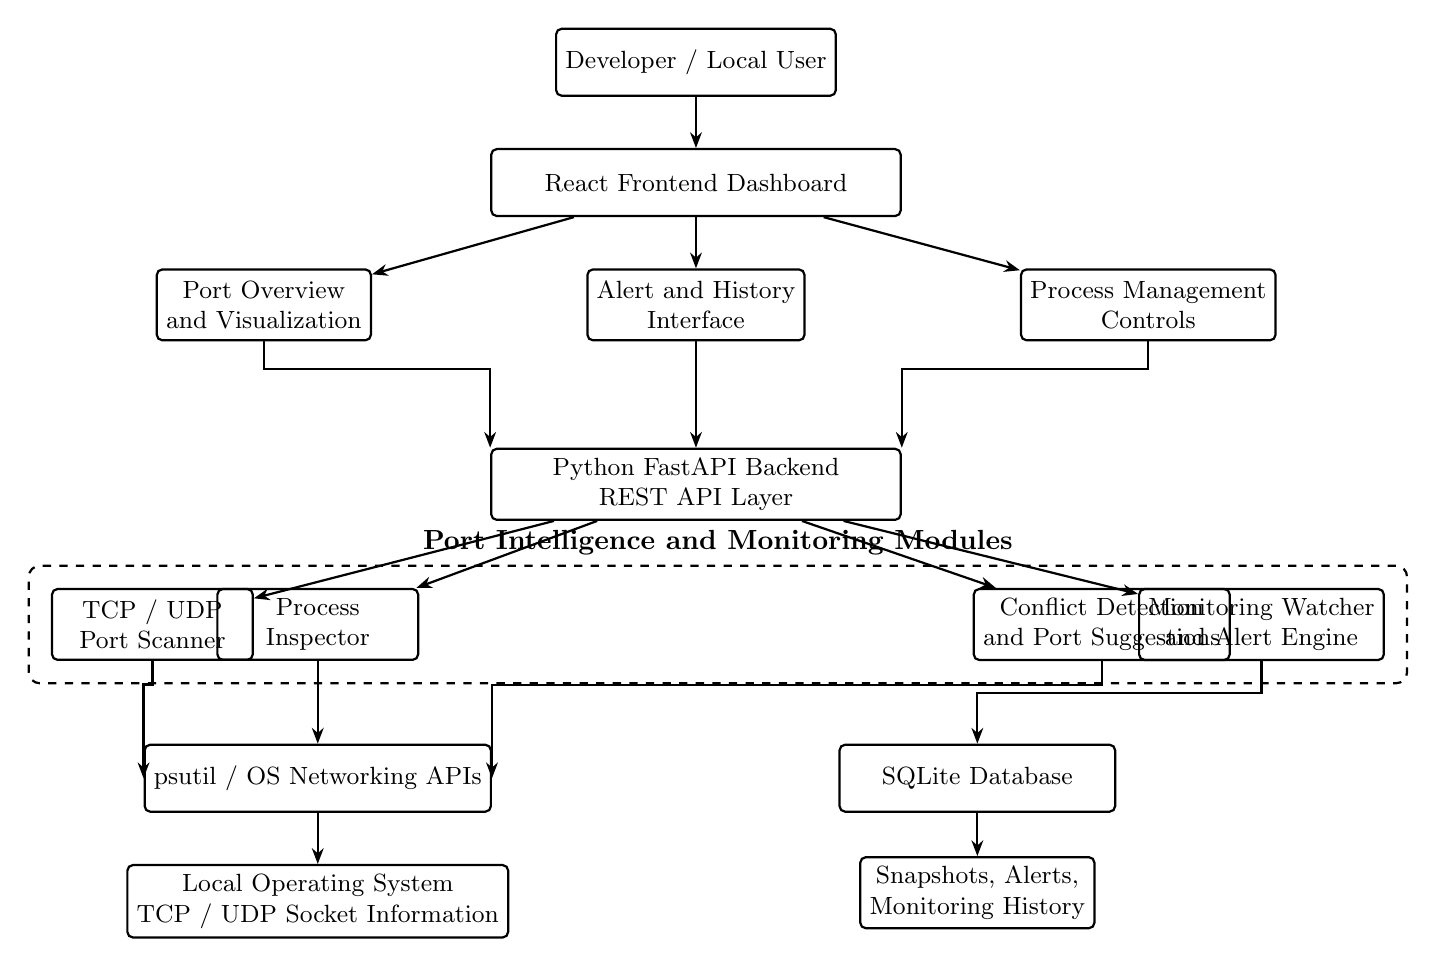
\begin{tikzpicture}[
    font=\small,
    block/.style={
        draw=black,
        rounded corners=2pt,
        thick,
        minimum width=3.0cm,
        minimum height=0.85cm,
        align=center
    },
    module/.style={
        draw=black,
        rounded corners=2pt,
        thick,
        minimum width=2.55cm,
        minimum height=0.9cm,
        align=center
    },
    arrow/.style={
        -{Stealth[length=2mm]},
        thick
    },
    boundary/.style={
        draw=black,
        dashed,
        rounded corners=4pt,
        thick,
        inner sep=8pt
    }
]

% User
\node[block, minimum width=3.5cm] (user)
{Developer / Local User};

% Frontend
\node[block, below=0.65cm of user,
minimum width=5.2cm] (frontend)
{React Frontend Dashboard};

\node[module, below left=0.65cm and 1.5cm of frontend] (dashboard)
{Port Overview\\and Visualization};

\node[module, below=0.65cm of frontend] (alerts)
{Alert and History\\Interface};

\node[module, below right=0.65cm and 1.5cm of frontend] (controls)
{Process Management\\Controls};

% Backend API
\node[block, below=1.35cm of alerts,
minimum width=5.2cm] (api)
{Python FastAPI Backend\\REST API Layer};

% Core modules
\node[module, below left=0.85cm and 3.0cm of api] (scanner)
{TCP / UDP\\Port Scanner};

\node[module, below left=0.85cm and 0.9cm of api] (inspector)
{Process\\Inspector};

\node[module, below right=0.85cm and 0.9cm of api] (conflict)
{Conflict Detection\\and Port Suggestions};

\node[module, below right=0.85cm and 3.0cm of api] (watcher)
{Monitoring Watcher\\and Alert Engine};

% System layer
\node[block, below=1.05cm of inspector,
minimum width=3.3cm] (psutil)
{psutil / OS Networking APIs};

\node[block, below=0.65cm of psutil,
minimum width=3.3cm] (os)
{Local Operating System\\TCP / UDP Socket Information};

% Database
\node[block, right=4.4cm of psutil,
minimum width=3.5cm] (database)
{SQLite Database};

\node[module, below=0.55cm of database] (records)
{Snapshots, Alerts,\\Monitoring History};

% User to frontend
\draw[arrow] (user) -- (frontend);

% Frontend internal interactions
\draw[arrow] (frontend) -- (dashboard);
\draw[arrow] (frontend) -- (alerts);
\draw[arrow] (frontend) -- (controls);

% Frontend to API
\draw[arrow] (dashboard.south) -- ++(0,-0.35) -| (api.north west);
\draw[arrow] (alerts.south) -- (api.north);
\draw[arrow] (controls.south) -- ++(0,-0.35) -| (api.north east);

% API to modules
\draw[arrow] (api) -- (scanner);
\draw[arrow] (api) -- (inspector);
\draw[arrow] (api) -- (conflict);
\draw[arrow] (api) -- (watcher);

% Modules to system layer
\draw[arrow] (scanner.south) -- ++(0,-0.3) -| (psutil.west);
\draw[arrow] (inspector.south) -- (psutil.north);
\draw[arrow] (conflict.south) -- ++(0,-0.3) -| (psutil.east);

% OS information
\draw[arrow] (psutil) -- (os);

% Monitoring to database
\draw[arrow] (watcher.south) -- ++(0,-0.4) -| (database.north);

\draw[arrow] (database) -- (records);

% Dashed subsystem boundary
\begin{scope}[on background layer]
\node[boundary,
fit=(scanner)(inspector)(conflict)(watcher),
label={[font=\bfseries]above:Port Intelligence and Monitoring Modules}
] {};
\end{scope}

\end{tikzpicture}

\caption{Modular architecture of the PortSentinel local port
monitoring and process intelligence system.}
\label{fig:architecture}

\end{figure*}

\subsection{Frontend Dashboard}

The frontend is developed using React and Tailwind CSS.
It provides a centralized interface for inspecting
local port utilization and displaying monitoring data.

The dashboard presents port information, process
details, alerts, historical records, and monitoring
summaries.

Recharts is used for graphical visualization of
available monitoring data.

\subsection{FastAPI Backend}

The backend is implemented using Python and FastAPI.

It acts as the central communication layer between
the frontend, system inspection modules, conflict
detection logic, and persistent storage.

The backend exposes endpoints for port scanning,
process information, conflict analysis, alert handling,
and monitoring history.

\subsection{Port Scanning Module}

The port scanning module collects local TCP and UDP
socket information using operating-system networking
interfaces and psutil.

Collected information includes:

\begin{itemize}
    \item Local IP address.
    \item Local port number.
    \item Transport protocol.
    \item Connection or socket state.
    \item Associated process identifier, when available.
\end{itemize}

The module is intended for local system inspection,
not unrestricted remote network scanning.

\subsection{Process Inspector}

The process inspector associates available process
identifiers with process metadata.

The information may include process names and
identification details exposed by the operating
system.

Process information can be incomplete when the
current user lacks the necessary permissions.

\subsection{Conflict Detection Engine}

The conflict detection engine analyzes the collected
port information to identify potential local port
conflicts.

It evaluates requested ports against currently
observed local socket usage and produces conflict
information for the dashboard.

The system can also suggest alternative candidate
ports based on the availability observed during
the inspection.

A suggested port must still be checked when the
application attempts to bind it, because port
availability can change between inspection and use.

\subsection{Monitoring and Alert Engine}

The monitoring component periodically collects
port information and compares observations with
previous snapshots.

The system can identify newly observed listeners
and generate corresponding monitoring alerts.

Users can review and acknowledge alerts through
the dashboard.

\subsection{SQLite Storage}

SQLite is used to maintain local application records.

The database stores monitoring snapshots, alert
records, and historical information used by the
dashboard.

This allows users to inspect previous monitoring
observations rather than relying only on the
current system state.

% =====================================================
% V. IMPLEMENTATION
% =====================================================
\section{Implementation}

\subsection{Technology Stack}

The principal technologies used in the project are
summarized in Table~\ref{tab:stack}.

\begin{table}[!t]
\centering
\caption{PortSentinel Technology Stack}
\label{tab:stack}

\begin{tabular}{|p{0.34\columnwidth}|p{0.54\columnwidth}|}
\hline
\textbf{Component} & \textbf{Technology}\\
\hline
Backend & Python, FastAPI\\
\hline
System Inspection & psutil, OS networking APIs\\
\hline
Frontend & React\\
\hline
Styling & Tailwind CSS\\
\hline
Visualization & Recharts\\
\hline
Database & SQLite\\
\hline
API Communication & REST\\
\hline
\end{tabular}
\end{table}

\subsection{Port Inspection Workflow}

The port inspection workflow begins when a user
requests a scan from the dashboard.

The frontend sends a request to the backend.
The backend collects the available local socket
information and processes the results.

The process inspector enriches the records with
process details when available.

The processed records are returned to the frontend
for presentation.

\subsection{Conflict Analysis}

The conflict detection module evaluates local port
usage against the port requested by an application.

A potential conflict is reported when the requested
port is already observed as occupied in the relevant
local binding context.

The system provides candidate alternative ports
based on the available inspection results.

\subsection{Historical Monitoring}

Monitoring snapshots are maintained in SQLite.

The monitoring component compares successive
observations to identify newly detected listening
services.

Alert records are maintained so that users can
review and acknowledge previously detected events.

\subsection{Process Management}

The project includes guarded process-management
operations.

These operations are intended to allow users to
manage selected processes through the dashboard.

Process-management actions require careful handling
because process termination may affect unrelated
applications or system services.

% =====================================================
% VI. METHODOLOGY
% =====================================================
\section{Development Methodology}

PortSentinel was developed using an incremental
implementation approach.

The development process was divided into the
following stages:

\begin{enumerate}
    \item Establish the backend API and local
    networking inspection functionality.
    \item Implement process identification and
    port conflict analysis.
    \item Develop alternative port recommendation
    logic.
    \item Introduce monitoring snapshots and
    alert generation.
    \item Implement the React dashboard and
    historical data presentation.
    \item Add guarded process-management
    functionality.
    \item Perform backend tests and integration
    checks.
\end{enumerate}

The modular development approach allowed the
backend functionality to be tested independently
before connecting it to the frontend.

% =====================================================
% VII. TESTING AND RESULTS
% =====================================================
\section{Testing and Results}

Testing was performed during the development of
the PortSentinel backend.

The project record reports four passing backend
tests.

The reported test coverage includes core backend
functionality. The complete React production build
and comprehensive Windows/Linux integration
behavior have not been independently verified.

\begin{table}[!t]
\centering
\caption{Reported Development Validation}
\label{tab:testing}

\begin{tabular}{|p{0.59\columnwidth}|c|}
\hline
\textbf{Validation Area} & \textbf{Result}\\
\hline
Backend test suite & 4 passed\\
\hline
TCP / UDP inspection logic & Implemented\\
\hline
Process identification & Implemented\\
\hline
Conflict detection & Implemented\\
\hline
Alternative port suggestions & Implemented\\
\hline
Monitoring snapshots & Implemented\\
\hline
Alert acknowledgement & Implemented\\
\hline
SQLite history & Implemented\\
\hline
Guarded process management & Implemented\\
\hline
Frontend production build & Not verified\\
\hline
Full cross-platform integration & Not verified\\
\hline
\end{tabular}
\end{table}

The results demonstrate the implementation of the
main backend modules and their reported test
coverage.

No numerical performance, detection-accuracy,
or scalability claims are made because a
reproducible benchmark dataset and measurement
results are not currently available.

% =====================================================
% VIII. DISCUSSION
% =====================================================
\section{Discussion}

PortSentinel combines several capabilities that
are commonly performed using separate system
utilities.

Its primary contribution is the integration of
local port inspection, process identification,
conflict analysis, monitoring history, and
interactive visualization into a single application.

The separation between the backend and frontend
allows system-level inspection to remain independent
of dashboard presentation.

The use of SQLite provides a lightweight mechanism
for storing historical monitoring records.

However, the reliability of system-wide process
identification depends on the permissions and
capabilities provided by the host operating system.

Furthermore, a port observed as available during
a scan may become occupied before another process
attempts to bind it. Therefore, recommendations
represent observations rather than guaranteed
reservations.

% =====================================================
% IX. LIMITATIONS AND FUTURE WORK
% =====================================================
\section{Limitations and Future Work}

The current implementation is primarily designed
for local development environments.

Several areas require additional investigation:

\begin{itemize}

    \item Comprehensive cross-platform validation
    on Windows and Linux.

    \item More extensive frontend and backend
    integration testing.

    \item Benchmarking scan latency and monitoring
    overhead.

    \item Improved handling of permission-restricted
    process information.

    \item More robust monitoring scheduling and
    failure recovery.

    \item Concurrency-safe process management
    and user confirmation.

    \item Improved port recommendation strategies.

    \item Extended historical analysis and
    visualization.

\end{itemize}

Future development may also investigate configurable
monitoring intervals, service identification,
container-aware process inspection, and more
advanced local development environment diagnostics.

% =====================================================
% X. CONCLUSION
% =====================================================
\section{Conclusion}

This paper presented PortSentinel, an intelligent
local port conflict monitoring and process
intelligence system designed for software
development environments.

The system integrates TCP and UDP socket inspection,
process identification, conflict detection,
alternative port suggestions, monitoring snapshots,
alert management, and historical storage.

Its modular architecture combines a Python FastAPI
backend, psutil-based operating-system inspection,
a React dashboard, and SQLite persistence.

The reported development results include four
passing backend tests and implementation of the
principal monitoring modules.

Further work is required to establish comprehensive
cross-platform reliability, frontend build validation,
and quantitative performance characteristics.

PortSentinel provides a foundation for improving
local port visibility and simplifying the
investigation of application startup conflicts.

% =====================================================
% REFERENCES
% =====================================================
\begin{thebibliography}{20}

\bibitem{tcp}
J. Postel,
``Transmission Control Protocol,''
RFC 793, Internet Engineering Task Force,
September 1981.
Available: \url{https://www.rfc-editor.org/rfc/rfc793}.

\bibitem{rfc9293}
W. Eddy, Ed.,
``Transmission Control Protocol (TCP),''
RFC 9293, Internet Engineering Task Force,
August 2022.
Available: \url{https://www.rfc-editor.org/rfc/rfc9293}.

\bibitem{udp}
J. Postel,
``User Datagram Protocol,''
RFC 768, Internet Engineering Task Force,
August 1980.
Available: \url{https://www.rfc-editor.org/rfc/rfc768}.

\bibitem{ip}
J. Postel,
``Internet Protocol,''
RFC 791, Internet Engineering Task Force,
September 1981.
Available: \url{https://www.rfc-editor.org/rfc/rfc791}.

\bibitem{rfc1122}
R. Braden, Ed.,
``Requirements for Internet Hosts -- Communication Layers,''
RFC 1122, Internet Engineering Task Force,
October 1989.
Available: \url{https://www.rfc-editor.org/rfc/rfc1122}.

\bibitem{netstat}
The Open Group,
``netstat -- Network Status,''
POSIX Utilities Specification.
Available: \url{https://pubs.opengroup.org/onlinepubs/9699919799/}.

\bibitem{lsof}
V. Abell,
``lsof -- List Open Files,''
Available: \url{https://github.com/lsof-org/lsof}.

\bibitem{psutil}
G. Rodola,
``psutil: Cross-platform Process and System Utilities,''
Official Documentation.
Available: \url{https://psutil.readthedocs.io/}.

\bibitem{fastapi}
S. Ramírez,
``FastAPI Documentation,''
Available: \url{https://fastapi.tiangolo.com/}.

\bibitem{sqlite}
SQLite Project,
``SQLite Transaction Documentation,''
Available: \url{https://www.sqlite.org/lang_transaction.html}.

\bibitem{sqliteabout}
SQLite Project,
``About SQLite,''
Available: \url{https://www.sqlite.org/about.html}.

\bibitem{react}
Meta Open Source,
``React Documentation,''
Available: \url{https://react.dev/learn}.

\bibitem{tailwind}
Tailwind Labs,
``Tailwind CSS Documentation,''
Available: \url{https://tailwindcss.com/docs}.

\bibitem{recharts}
Recharts Contributors,
``Recharts: Composable Charting Library for React,''
Available: \url{https://recharts.org/}.

\bibitem{rest}
R. T. Fielding,
``Architectural Styles and the Design of Network-based
Software Architectures,''
Ph.D. dissertation, University of California,
Irvine, 2000.
Available: \url{https://www.ics.uci.edu/~fielding/pubs/dissertation/top.htm}.

\bibitem{http}
R. Fielding, M. Nottingham, and J. Reschke,
``HTTP Semantics,''
RFC 9110, Internet Engineering Task Force,
June 2022.
Available: \url{https://www.rfc-editor.org/rfc/rfc9110}.

\bibitem{socket}
W. R. Stevens,
\emph{TCP/IP Illustrated, Volume 1: The Protocols},
Addison-Wesley, 1994.

\bibitem{computer}
A. S. Tanenbaum and H. Bos,
\emph{Modern Operating Systems},
4th ed., Pearson, 2015.

\bibitem{network}
A. S. Tanenbaum and D. J. Wetherall,
\emph{Computer Networks},
5th ed., Pearson, 2011.

\bibitem{linux}
M. Kerrisk,
\emph{The Linux Programming Interface},
No Starch Press, 2010.

\end{thebibliography}

\end{document}
